\documentclass[DaoFP]{subfiles}
\begin{document}
\setcounter{chapter}{11}

\chapter{Coalgebras}

Coalgebras are just algebras in the opposite category. End of chapter!

Well, maybe not... As we've seen before, the category in which we're working is not symmetric with respect to duality. In particular, if we compare the terminal and the initial objects, their properties are not symmetric. Our initial object has no incoming arrows, whereas the terminal one, besides having unique incoming arrows, has lots of outgoing arrows. 

Since initial algebras were constructed starting from the initial object, we might expect terminal coalgebras---which are their duals, therefore generated from the terminal object---not to be just their mirror images, but to add their own interesting twists.

We've seen that the main application of algebras was in processing recursive data structures: in folding them. Dually, the main application of coalgebras is in generating, or unfolding, the recursive, tree-like, data structures. The unfolding is done using an anamorphism.

We use catamorphisms to chop trees, we use anamorphisms to grow them. 

We cannot produce information from nothing so, in general, both a catamorphism and an anamorphism tend to reduce the amount of information that's contained in their input. 

After you sum a list of integers, it's impossible to recover the original list. 

By the same token, if you grow a recursive data structure using an anamorphism, the seed must contain all the information that ends up in the tree. You don't gain new information, but the advantage is that the information you have is now stored in a form that's more convenient for further processing.

\section{Coalgebras from Endofunctors}

A coalgebra for an endofunctor $F$ is a pair consisting of a carrier $a$ and a structure map: an arrow $a \to F a$. 

In Haskell, we define:
\begin{haskell}
 type Coalgebra f a = a -> f a
\end{haskell}
We often think of the carrier as the type of a seed from which we grow the data structure, be it a list or a tree. 

For instance, here's a functor that can be used to create a binary tree, with integers stored at the nodes:
\begin{haskell}
data TreeF x = LeafF | NodeF Int x x
  deriving (Show, Functor)
\end{haskell}
We don't even have to define the instance of \hask{Functor} for it---the \hask{deriving} clause tells the compiler to generate the canonical one for us (together with the \hask{Show} instance to allow conversion to \hask{String}, if we want to display it).

A coalgebra is a function that takes a seed of the carrier type and produces a functorful of new seeds. These new seeds can then be used to generate the subtrees, recursively. 

Here's a coalgebra for the functor \hask{TreeF} that takes a list of integers as a seed:
\begin{haskell}
split :: Coalgebra TreeF [Int]
split [] = LeafF
split (n : ns) = NodeF n left right
  where
    (left, right) = partition (<= n) ns
\end{haskell}
If the seed is empty, it generates a leaf; otherwise it creates a new node. This node stores the head of the list and fills the node with two new seeds. The library function \hask{partition} splits a list using a user-defined predicate, here \hask{(<= n)}, less-than-or-equal to \hask{n}. The result is a pair of lists: the first one satisfying the predicate; and the second, not. 

You can convince yourself that a recursive application of this coalgebra creates a binary sorted tree. We'll use this coalgebra later to implement a sort.

\section{Category of Coalgebras}

By analogy with algebra morphisms, we can define coalgebra morphisms as the arrows between carriers that satisfy a commuting condition. 

Given two coalgebras $(a, \alpha)$ and $(b, \beta)$, the arrow $f \colon a \to b$ is a coalgebra morphism if the following diagram commutes:

\[
 \begin{tikzcd}
 a 
 \arrow[r, "f"]
 \arrow[d, "\alpha"]
 & b
\arrow[d, "\beta"]
 \\
F  a
 \arrow[r, "F f"]
 & F b
  \end{tikzcd}
\]

The interpretation is that it doesn't matter if we first map the carriers and then apply the coalgebra $\beta$, or first apply the coalgebra $\alpha$ and then apply the arrow to its contents, using the lifting $F f$.

Coalgebra morphisms can be composed, and the identity arrow is automaticaly a coalgebra morphism. It's easy to see that coalgebras, just like algebras, form a category. 

This time, however, we are interested in the terminal object in this category---a \emph{terminal coalgebra}. If a terminal coalgebra $(t, \tau)$ exists, it satisfies the dual of the Lambek's lemma. 

\begin{exercise}{Lambek's lemma:}
Show that the structure map $\tau$ of the terminal coalgebra $(t, \tau)$ is an isomorphism. Hint: The proof is dual to the one for the initial algebra.
\end{exercise}

As a consequence of the Lambek's lemma, the carrier of the terminal algebra is a fixed point of the endofunctor in question. 
\[ F t \cong t \]
with $\tau$ and $\tau^{-1}$ serving as the witnesses of this isomorphism. 

It also follows that $(t, \tau^{-1})$ is an algebra; just as  $(i, \iota^{-1})$ is a coalgebra, assuming that $(i, \iota)$ is the initial algebra.

We've seen before that the carrier of the initial algebra is a fixed point. In principle, there may be many fixed points for the same endofunctor. The initial algebra is the least fixed point and the terminal coalgebra the greatest fixed point. 

The greatest fixed point of an endofunctor $F$ is denoted by $\nu F$, so we have:
\[ t = \nu F \]

We can also see that there must be a unique algebra morphism (a catamorphism) from the initial algebra to the terminal coalgebra. That's because the terminal coalgebra is also an algebra. 

Similarly, there is a unique coalgebra morphism from the initial algebra (which is also a coalgebra) to the terminal coalgebra. In fact, it can be shown that it's the same underlying morphism $\rho \colon \mu F \to \nu F$ in both cases. 

In the category of sets, the carrier set of the initial algebra is a subset of the carrier set of the terminal coalgebra, with the function $\rho$ embedding the former in the latter. 
\[
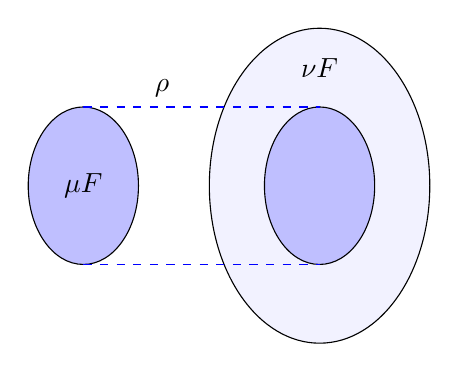
\begin{tikzpicture}
         \draw (-1,0)[fill=blue!25!white] ellipse (0.7 and 1);
         \draw (2,0)[fill=blue!5!white] ellipse (1.4 and 2);
         \draw (2,0)[fill=blue!25!white] ellipse (0.7 and 1);
         \node[above] at (0, 1) {$\rho$};
       	\draw[dashed, blue] (-1, 1) -- (2, 1);
	\draw[dashed, blue] (-1, -1) -- (2, -1);
        \node at (-1, 0) { $\mu F$ };
        \node at (2, 1.5) { $\nu F$ };
\end{tikzpicture}
\]

We'll see later that in Haskell the situation is more subtle, because of lazy evaluation. But, at least for functors that have the leaf component---that is, their action on the initial object is non-trivial---Haskell's fixed point type works as a carrier for both the initial algebra and the terminal coalgebra.
\begin{haskell}
data Fix f where
  In :: f (Fix f) -> Fix f
\end{haskell}

\begin{exercise}
Show that, for the identity functor in $\mathbf{Set}$, every object is a fixed point, the empty set is the least fixed point, and the singleton set is the greatest fixed point. Hint: The least fixed point must have arrows going to all other fixed points, and the greatest fixed point must have arrows coming from all other fixed points.
\end{exercise}

\begin{exercise}
Show that the empty set is the carrier of the initial algebra for the identity functor in $\mathbf{Set}$. Dually, show that the singleton set is this functor's terminal coalgebra. Hint: Show that the unique arrows are indeed (co-) algebra morphisms.
\end{exercise}

\section{Anamorphisms}

The terminal coalgebra $(t, \tau)$ is defined by its universal property: there is a unique coalgebra morphism $h$ from any coalgebra $(a, \alpha)$ to $(t, \tau)$.  This morphism is called the \emph{anamorphism}. Being a coalgebra morphism, it makes the following diagram commute:
\[
 \begin{tikzcd}
 a 
 \arrow[r, dashed, "h"]
 \arrow[d, "\alpha"]
 & t
\arrow[d, "\tau"]
 \\
 F a
 \arrow[r,  "F h"]
 & F t
  \end{tikzcd}
\]
 
 Just like with algebras, we can use the Lambek's lemma to ``solve'' for \hask{h}:
 \[ h = \tau^{-1} \circ F h \circ \alpha \]
 The solution is called an anamorphism and is sometimes written using \index{lens bracket}\index{$\llens \rlens$}``lens brackets'' as $\llens \alpha \rlens$.
 
 Since the terminal coalgebra (just like the initial algebra) is a fixed point of a functor, the above recursive formula can be translated directly to Haskell as:
 \begin{haskell}
ana :: Functor f => Coalgebra f a -> a -> Fix f
ana coa = In . fmap (ana coa) . coa 
\end{haskell}
Here's the interpretation of this formula: Given a seed of type \hask{a}, we first act on it with the coalgebra \hask{coa}. This gives us a functorful of seeds. We expand these seeds by recursively applying the anamorphism using \hask{fmap}. We then apply the constructor \hask{In} to get the final result.
 
As an example, we can apply the anamorphism to the \hask{split} coalgebra we defined earlier: \hask{ana split} takes a list of integers and creates a sorted tree. 

We can then use a catamorphsims to fold this tree into a sorted list. We define the following algebra:
\begin{haskell}
toList :: Algebra TreeF [Int]
toList LeafF = []
toList (NodeF n ns ms) = ns ++ [n] ++ ms
\end{haskell}
It concatenates the left list with the singleton pivot and the right list. To sort a list we combine the anamorphism with the catamorphism:
\begin{haskell}
qsort = cata toList . ana split
\end{haskell}
This gives us a (very inefficient) implementation of quicksort. We'll come back to it in the next section.

\subsection{Infinite data structures}

When studying algebras we relied on data structures that had a leaf component---that is endofunctors that, when acting on the initial object, would produce a result different from the initial object. When constructing recursive data structures we had to start somewhere, and that meant constructing the leaves first.

With coalgebras, we are free to drop this requirement. We no longer have to construct recursive data structures ``by hand''---we have anamorphisms to do that for us. An endofunctor that has no leaves is perfectly acceptable: its coalgebras are going to generate infinite data structures. 

Infinite data structures are representable in Haskell because of its laziness. Things are evaluated on the need-to-know basis. Only those parts of an infinite data structure that are explicitly demanded are calculated; the evaluation of the rest is kept in suspended animation. 

To implement infinite data structures in strict languages, one must resort to representing values as functions---something Haskell does behind the scenes (these functions are called \emph{thunks}).

Let's look at a simple example: an infinite stream of values. To generate it, we first define a functor that looks very much like the one we used to generate lists, except that it lacks the leaf component (the empty-list constructor). You may recognize it as a product functor, with the first component fixed to be the stream's payload:
\begin{haskell}
data StreamF a x = StreamF a x
  deriving Functor
\end{haskell}
An infinite stream is the fixed point of this functor.
\begin{haskell}
type Stream a = Fix (StreamF a)
\end{haskell}
Here's a simple coalgebra that uses a single integer \hask{n} as a seed:
\begin{haskell}
step :: Coalgebra (StreamF Int) Int
step n = StreamF n (n+1)
\end{haskell}
It stores the current seed as a payload, and seeds the next budding stream with \hask{n + 1}. 

The anamorphism for this coalgebra, when seeded with zero, generates the stream of all natural numbers.
\begin{haskell}
allNats :: Stream Int
allNats = ana step 0
\end{haskell}
In a non-lazy language this anamorphism would run forever, but in Haskell it's instantaneous. The incremental price is paid only when we want to retrieve some of the data, for instance, using these accessors:
\begin{haskell}
head :: Stream a -> a
head (In (StreamF a _)) = a

tail :: Stream a -> Stream a
tail (In (StreamF _ s)) = s
\end{haskell}


\section{Hylomorphisms}

The type of the output of an anamorphism is a fixed point of a functor, which is the same type as the input to a catamorphism. In Haskell, they are both described by the same data type, \hask{Fix f}. Therefore it's possible to compose them together, as we've done when implementing quicksort. In fact, we can combine a coalgebra with an algebra in one recursive function called a \emph{hylomorphism}:
\begin{haskell}
hylo :: Functor f => Algebra f b -> Coalgebra f a -> a -> b
hylo alg coa = alg . fmap (hylo alg coa) . coa 
\end{haskell}
We can rewrite quicksort as a hylomorphism:
\begin{haskell}
qsort = hylo toList split
\end{haskell}

Notice that there is no trace of the fixed point in the definition of the hylomorphism. Conceptually, the coalgebra is used to build (unfold) the recursive data structure from the seed, and the algebra is used to fold it into a value of type \hask{b}. But because of Haskell's laziness, the intermediate data structure doesn't have to be materialized in full in memory. This is particularly important when dealing with very large intermediate trees. Only the branches that are currently being traversed are evaluated and, as soon as they have been processed, they are passed to the garbage collector. 

Hylomorphisms in Haskell are a convenient replacement for recursive backtracking algorithms, which are very hard to implement correctly in imperative languages. We take advantage of the fact that designing a data structure is easier than following complicated flow of control and keeping track of our place in a recursive algorithm. 

This way, data structures can be used to visualize complex flows of control.

\subsection{The impedance mismatch}
We've seen that, in the category of sets, the initial algebras don't necessarily coincide with terminal coalgebras. The identity functor, for instance, has the empty set as the carrier of the initial algebra and the singleton set as the carrier of its terminal coalgebra. 

We have other functors that have no leaf components, such as the stream functor. The initial algebra for such a functor is the empty set as well. 

In $\mathbf{Set}$, the initial algebra is the subset of the terminal coalgebra, and hylomorphisms can only be defined for this subset. It means that we can use a hylomorphism only if the anamorphism for a particular coalgebra lands us in this subset. In that case, because the embedding of initial algebras in terminal coalgebras is injective, we can find the corresponding element in the initial algebra and apply the catamorphism to it.

In Haskell, however, we have one type, \hask{Fix f}, combining both, the initial algebra and the terminal coalgebra. This is where the simplistic interpretation of Haskell types as sets of values breaks down. 

Let's consider this simple stream algebra:
\begin{haskell}
add :: Algebra (StreamF Int) Int
add (StreamF n sum) = n + sum
\end{haskell}
Nothing prevents us from using a hylomorphism to calculate the sum of all natural numbers:
\begin{haskell}
sumAllNats :: Int
sumAllNats = hylo add step 1
\end{haskell}
It's a perfectly well-formed Haskell program that passes the type checker. So what value does it produce when we run it? (Hint: It's not $-1/12$.) The answer is: we don't know, because this program never terminates. It runs into infinite recursion and eventually exhausts the computer's resources.

This is the aspect of real-life computations that mere functions between sets cannot model. Some computer function may never terminate. 

Recursive functions are formally described by \emph{domain theory} as limits of partially defined functions. If a function is not defined for a particular value of the argument, it is said to return a bottom value $\bot$. If we include bottoms as special elements of every type (these are then called \index{lifted types}\emph{lifted} types), we can say that our function \hask{sumAllNats} returns a bottom of the type \hask{Int}. In general, catamorphisms for infinite types don't terminate, so we can treat them as returning bottoms.

It should be noted, however, that the inclusion of bottoms complicates the categorical interpretation of Haskell. In particular, many of the universal constructions that rely on uniqueness of mappings no longer work as advertised.

The ``bottom'' line is that Haskell code should be treated as an illustration of categorical concepts rather than a source of rigorous proofs.

\section{Terminal Coalgebra from Universality}

The definition of an anamorphism can be seen as an expression of the universal property of the terminal coalgebra. Here it is, with the universal quantification made explicit:
 \begin{haskell}
ana :: Functor f => forall a. Coalgebra f a -> (a -> Fix f)
ana coa = In . fmap (ana coa) . coa 
\end{haskell}
What it tells us is that, given any coalgebra, there is a mapping from its carrier to the carrier of the terminal coalgebra, \hask{Fix f}. We know, from the Lambek's lemma, that this mapping is in fact a coalgebra morphism.

Let's uncurry this definition:
\begin{haskell}
ana :: Functor f => forall a. (a -> f a, a) -> Fix f
ana (coa, x) = In (fmap (curry ana coa) (coa x))
\end{haskell}
We can use this formula as the alternative definition of the carrier for the terminal coalgebra. We can replace \hask{Fix f} with the type we are defining---let's call it \hask{Nu f}. The type signature:
\begin{haskell}
forall a. (a -> f a, a) -> Nu f
\end{haskell}
tells us that we can construct an element of \hask{Nu f} from a pair \hask{(a -> f a, a)}. It looks just like a data constructor, except that it's polymorphic in \hask{a}. 

Data types with a polymorphic constructor are called \index{existential types}\emph{existential} types. In pseudo-code (not actual Haskell) we would define \hask{Nu f} as:
\begin{haskell}
data Nu f = Nu (exists a. (Coalgebra f a, a))
\end{haskell}
Compare this with the definition of the least fixed point of an algebra:
\begin{haskell}
data Mu f = Mu (forall a. Algebra f a -> a)
\end{haskell}


To construct an element of an existential type, we have the option of picking the most convenient type---the type for which we have the data required by the constructor. 

For instance, we can construct a term of the type \hask{Nu (StreamF Int)} by picking \hask{Int} as the convenient type, and providing the pair:
\begin{haskell}
nuArgs :: (Int -> StreamF Int Int, Int)
nuArgs =  (\n -> StreamF n (n+1) , 0)
\end{haskell}

The clients of an existential data type have no idea what type was used in its construction. All they know is that such a type \emph{exists}---hence the name. If they want to use an existential type, they have to do it in a way that is not sensitive to the choice that was made in its construction. In practice, it means that an existential type must carry with itself both the producer and the consumer of the hidden value. 

This is indeed the case in our example: the producer is just the value of type \hask{a}, and the consumer is the function \hask{a -> f a}.

Naively, all that the clients could do with this pair, without any knowledge of what the type \hask{a} was, is to apply the function to the value. But if \hask{f} is a functor, they can do much more. They can repeat the process by applying the lifted function to the contents of \hask{f a}, and so on. They end up with all the information that's contained in the infinite stream.

There are several ways of defining existential data types in Haskell. We can use the uncurried version of the anamorphism directly as the data constructor:
\begin{haskell}
data Nu f where 
  Nu :: forall a f. (a -> f a, a) -> Nu f
\end{haskell}
Notice that, in Haskell, if we explicitly quantify one type, all other type variables must also be quantified: here, it's the type constructor \hask{f} (however, \hask{Nu f} is not existential in \hask{f}, since it's an explicit parameter). 

We can also omit the quantification altogether:
\begin{haskell}
data Nu f where 
  Nu :: (a -> f a, a) -> Nu f
\end{haskell}
This is because type variables that are not arguments to the type constructor are automatically treated as existentials. 

We can also use the more traditional form:
\begin{haskell}
data Nu f = forall a. Nu (a -> f a, a)
\end{haskell}
(This one requires the quantification of \hask{a}.)

At the time of this writing there is a proposal to introduce the keyword \hask{exists} to Haskell that would make this definition work:
\begin{haskell}
data Nu f = Nu (exists a. (a -> f a, a))
\end{haskell}
(Later we'll see that existential data types correspond to coends in category theory.)

The constructor of \hask{Nu f} is literally the (uncurried) anamorphism:
\begin{haskell}
anaNu :: Coalgebra f a -> a -> Nu f
anaNu coa a = Nu (coa, a)
\end{haskell}

If we are given a stream in the form of \hask{Nu (Stream a)}, we can access its element using accessors functions. This one extracts the first element:
\begin{haskell}
head :: Nu (StreamF a) -> a
head (Nu (unf, s)) = 
  let (StreamF a _) = unf s 
  in a
\end{haskell}
and this one advances the stream:
\begin{haskell}
tail :: Nu (StreamF a) -> Nu (StreamF a)
tail (Nu (unf, s)) = 
  let (StreamF _ s') = unf s 
  in Nu (unf, s')
\end{haskell}
You can test them on an infinite stream of integers:
\begin{haskell}
allNats = Nu nuArgs
\end{haskell}

\section{Terminal Coalgebra as a Limit}

In category theory we are not afraid of infinities---we make sense of them. 

At face value, the idea that we could construct a terminal coalgebra by applying the functor $F$ infinitely many times to some object, let's say the terminal object $1$, makes no sense. But the idea is very convincing: Applying $F$ one more time is like adding one to infinity---it's still infinity. So, naively, this is a fixed point of $F$:
\[ F (F^{\infty} 1) \cong F^{\infty + 1} 1 \cong F^{\infty} 1\]

To turn this loose reasoning into a rigorous proof, we have to tame the infinity, which means we have to define some kind of limiting procedure. 

As an example, let's consider the product functor:
\[F_a x = a \times x \]
Its terminal coalgebra is an infinite stream. We'll approximate it by starting with the terminal object $1$. The next step is:
\[ F_a 1 = a \times 1 \cong a \]
which we could imagine is a stream of length one. We can continue with:
\[ F_a (F_a 1) = a \times (a \times 1) \cong a \times a \]
a stream of length two, and so on. 

This looks promising, but what we need is one object that would combine all these approximations. We need a way to glue the next approximation to the previous one.

Recall, from an earlier exercise, the limit of the ``walking arrow'' diagram. This limit has the same elements as the starting object in the diagram. In particular, consider the limit of the single-arrow diagram $D_1$:
\[
 \begin{tikzcd}
 & Lim D_1
 \arrow[dl, "\pi_0"']
\arrow[d, "\pi_1"]
 \\
 1 
 & F1
 \arrow[l, "!"]
 \end{tikzcd}
\]
($!$ is the unique morphism targeting the terminal object $1$). This limit has the same elements as $F 1$. Similarly, the limit of a two-arrow diagram $D_2$:
\[
 \begin{tikzcd}
 && Lim D_2
 \arrow[dll, "\pi_0"']
\arrow[dl, "\pi_1"]
\arrow[d, "\pi_2"]
 \\
 1 
 & F1
 \arrow[l, "!"]
  & F(F 1)
 \arrow[l, "F !"]
\end{tikzcd}
\]
has the same elements as $F(F 1)$.

We can continue extending this diagram to infinity. It turns out that the limit of this infinite chain is our fixed point carrier of the terminal coalgebra.
\[
 \begin{tikzcd}
  && t
  \arrow[ddll, "\pi_0"']
  \arrow[ddl, "\pi_1"]
  \arrow[dd, "\pi_2"]
  \arrow[ddrr, "\pi_n"]
\\
\\
 1 
 & F 1
 \arrow[l, "!"]
 & F (F 1)
 \arrow[l, "F !"]
 & ...
 \arrow[l, "F(F !)"]
 & F^n 1
  \arrow[l]
 & ...
  \arrow[l, "F^n !"]
 \end{tikzcd}
\]
The proof of this fact can be obtained from the analogous proof for initial algebras by reversing the arrows.

\end{document}